\renewcommand{\theequation}{\theenumi}
\begin{enumerate}[label=\arabic*.,ref=\thesubsection.\theenumi]
\numberwithin{equation}{enumi}

\item 
Let assume that we have a point $\vec{C}\myvec{x\\0}$ which devide the linesegment $\vec{AB} $ in k:1 ratio.

\begin{align}
\left(k+1\right)\myvec{x\\0} &=k\myvec{1\\-5} + \myvec{-4\\5}
\\
0 &= -5k + 5
\\
k&= 1
\\
\vec{C} &= \frac{\myvec{-3\\0}}{2} 
\\&= \myvec{-1.5\\0}
\end{align}
\begin{figure}[!ht]
	\centering
	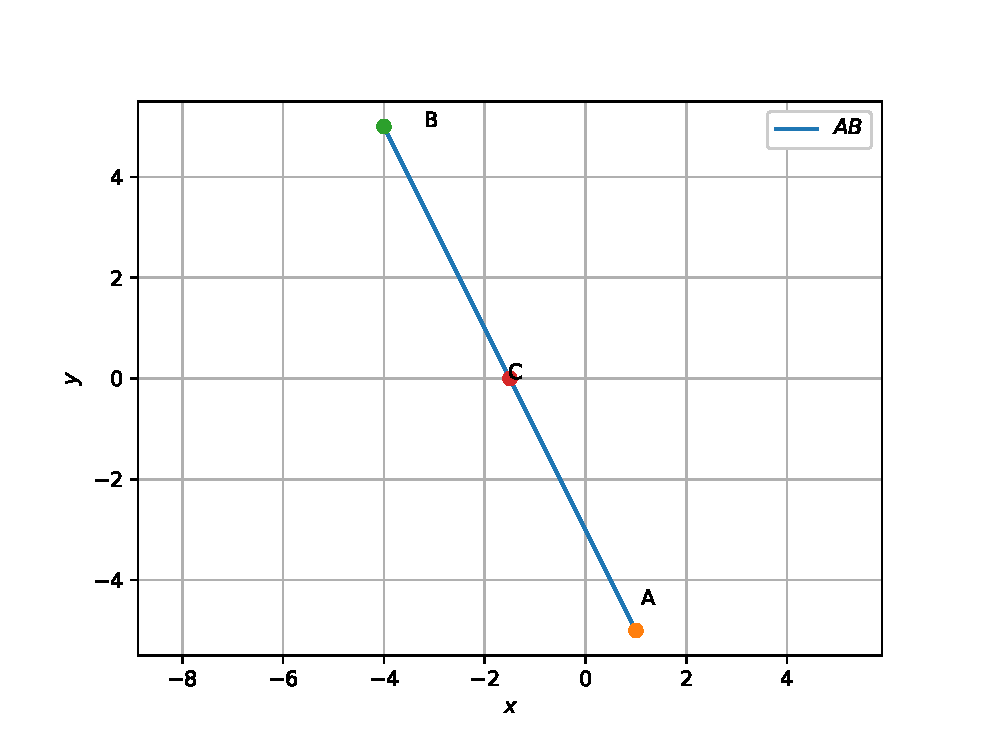
\includegraphics[width=\columnwidth]{./figures/line/point_on_line/point_on_line.eps}
	\caption{line }
	\label{fig:line}
	path to the python code for the above figure 
	\begin{lstlisting}
	codes/line/point_on_line/points_on_line.py
	\end{lstlisting}
\end{figure}


\end{enumerate}